\chapter{Organización}
\section{Introducción}
\newpage
\section{PROPIEDAD HORIZONTAL}

\subsection{Misión}

Lograr que todos los copropietarios acaten las normas de convivencia en la propiedad horizontal con respeto y responsabilidad, con el fin de llegar a disfrutar cada día una mejor alternativa de vivienda beneficiando su calidad de vida, la seguridad personal y satisfacción de sus necesidades básicas de bienestar. Siempre liderando con un alto sentido de calidad, respeto y responsabilidad hasta alcanzar la total satisfacción de los habitantes.

\subsection{Visión}

La propiedad horizontal será un modelo de calidad de vida y sana convivencia, que garantice auto sostenibilidad a nivel local regional, con excelentes desempeños en todas las dimensiones de su vida en un contexto de interacción armónica donde el quehacer diario se sustente en los valores, la cultura y el respeto a los demás.


\subsection{Estructura Orgánica}


\begin{figure}[th!]
	\centering
	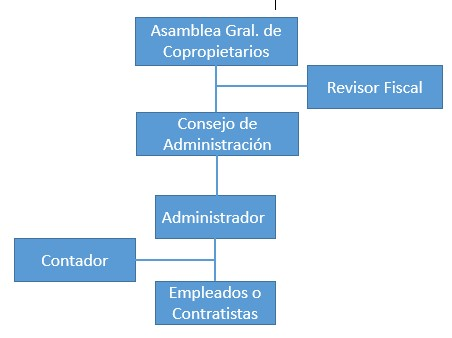
\includegraphics[width=0.7\linewidth]{arquitectura/organizacion/imgs/organigrama}
	\caption{Est. Organica}	
\end{figure}



\subsection{Manual de Funciones}

\subsubsection{Administrador}


\begin{itemize}
\item Convocar la asamblea.
\item Someter a aprobación el inventario.
\item Llevar la contabilidad del edificio.
\item Informar a los propietarios y residentes las decisiones de la asamblea.
\item Administrar los bienes de la propiedad horizontal.
\item Cuidar y vigilar los bienes comunes.
\item Cobrar y recaudar las multas y cuotas ordinarias y extraordinarias.
\item Representar judicial y extrajudicialmente.
\item Hacer efectivas las sanciones.
\item Expedir el paz y salvo de cuentas de la Administración.
\end{itemize}


\subsubsection{Consejo de Administración}
\begin{itemize}
\item Llevar propuestas a la asamblea acerca de reglamentos de usos de bienes comunes y de las modificaciones en la forma y goce de los mismos.
\item Proponer a la asamblea la realización de programas de mejoras de obras y reparaciones o la reconstrucción parcial o total del inmueble y la forma de distribución del costo entre propietarios.
\item Vigilar la administración el inmueble y dictar los reglamentos internos tendientes a que se mantenga el orden y el aseo en la copropiedad.
\item Autorizar al administrador para todos los actos de carácter extraordinario que se presenten.
\item Asesorar al administrador en todas las cuestiones relativas al mejor funcionamiento de la persona jurídica, ejercitar ampliamente el control de su gestión y cuando juzgue conveniente dar cuenta de ello a la asamblea general de propietarios.
\item Convocar a la asamblea a reunión ordinaria cuando el administrador no lo hubiere hecho oportunamente o cuando lo estime conveniente para las asambleas extraordinarias.
\item Presentar a la asamblea de propietarios informe de su gestión anual y el concepto acerca del proyecto de presupuesto anual de gastos que debe presentar el administrador a consideración de la asamblea.
\item Nombrar y remover libremente al administrador cuando sea una persona natural y fijarle su remuneración y supervisar sus funciones.
\item Imponer a los propietarios y demás ocupantes de la copropiedad, las sanciones por el incumplimiento de obligaciones no pecuniarias, en los casos en que la Asamblea le hubiere delegado tal responsabilidad y de conformidad con lo establecido en la ley y el reglamento de propiedad horizontal.
\item Velar por la correcta inversión de los fondos de imprevistos conforme a la destinación dada por la asamblea general.

\end{itemize}

\subsubsection{Revisor Fiscal}

\begin{itemize}
	
\item Cerciorarse de que las operaciones que se celebren o cumplan por cuenta de la propiedad horizontal se ajustan a las prescripciones de los estatutos, a las decisiones de la asamblea general y del consejo de administración.
\item Dar oportuna cuenta, por escrito, a la asamblea general al consejo e administración o al administrador, según los casos, de las irregularidades que ocurran en el funcionamiento de la propiedad horizontal;
\item Colaborar con las entidades gubernamentales que ejerzan la inspección y vigilancia de la propiedad horizontal, y rendirles los informes a que haya lugar o le sean solicitados;
\item Velar por que se lleven regularmente la contabilidad de la propiedad horizontal y las actas de las reuniones de la asamblea, del consejo de administración, y porque se conserven debidamente la correspondencia de la copropiedad y los comprobantes de las cuentas, impartiendo las instrucciones necesarias para tales fines;
\item Inspeccionar asiduamente los bienes de la propiedad horizontal y procurar que se tomen oportunamente las medidas de conservación o seguridad de los mismos y de los que ella tenga en custodia a cualquier otro título;
\item Impartir las instrucciones, practicar las inspecciones y solicitar los informes que sean necesarios para establecer un control permanente sobre los valores sociales;
\item Autorizar con su firma cualquier balance que se haga, con su dictamen o informe correspondiente;
\item Convocar a la asamblea o al consejo de administración a sesiones extraordinarias cuando lo juzgue necesario, y cumplir las demás atribuciones que le señalen las leyes o los estatutos y las que, siendo compatibles con las anteriores, le encomiende la asamblea o junta de socios.
\end{itemize}	

\subsection{Procesos Organizacionales}

\subsubsection{Procesos}

\begin{figure}[th!]
	\centering
	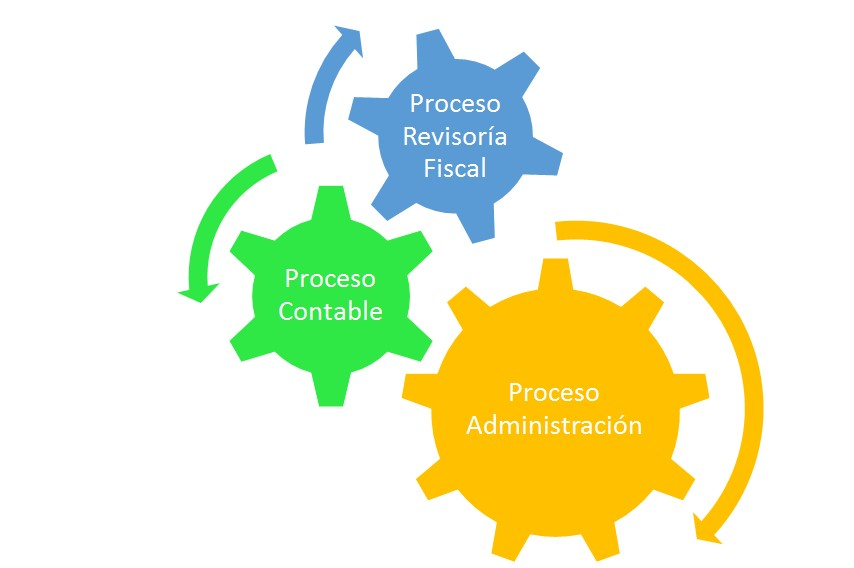
\includegraphics[width=0.7\linewidth]{arquitectura/organizacion/imgs/procesos_org1}
	\caption{Procesos Organizacionales}	
\end{figure}

\newpage

\subsubsection{Descripción}


\begin{figure}[th!]
	\centering
	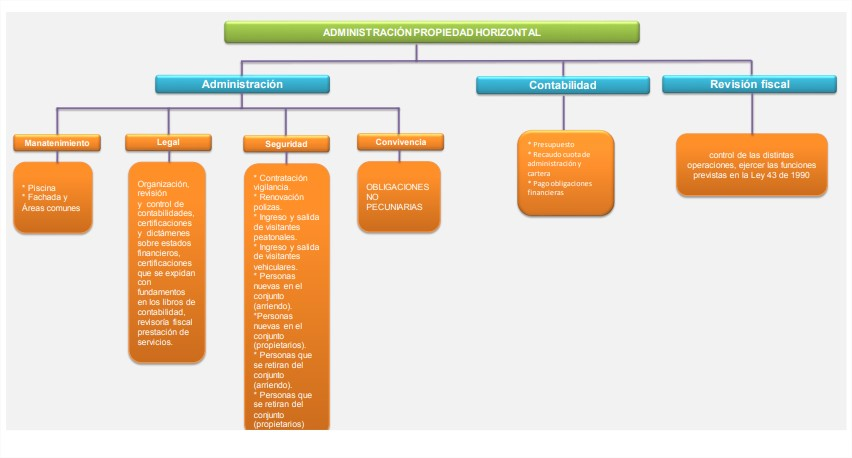
\includegraphics[width=0.7\linewidth]{arquitectura/organizacion/imgs/procesos_org2}
	\caption{Descripcion Procesos}
	
\end{figure}


\begin{itemize}
	
\item Administración: Permiten establecer reglas de protocolo que orienten la buena convivencia a través de criterios y procedimientos internos propios de la propiedad horizontal y que permitan generar un clima de sana convivencia de acuerdo a las normas establecidas, buscando acercamiento y entendimiento entre los copropietarios y también con la administración. Permiten conocer los procedimientos de convivencia que se deben desarrollar en la propiedad horizontal, teniendo en cuenta los lineamientos según la normativa que indique el cómo se debe atender a las necesidades, de esta forma lograr un óptimo resultado. 

\item Contabilidad: Procesos de administración que permitan el recaudo de las cuotas de administración y destinarlas a los rubros que se han determinado, estableciendo el responsable de este proceso que ayuden a tener el mejor manejo de este.

\item Revisión Fiscal: Efectuar el control y vigilancia la correcta ejecución de lo estipulado en el contrato con la Asamblea. Certificar la responsabilidad sobre los actos y decisiones que toma la administración ya que con su certificación busca la seguridad de los intereses de la comunidad de copropietarios y por ende el bienestar económico.
\end{itemize}

\subsection{Servicios y/o Productos}

\begin{itemize}
\item Servicio de vigilancia 7*24
\item Servicio de parqueadero
\item Alquiler salones comunales
\item Servicios generales (Aseo y mantenimiento) de zonas comunes
\item Gimnasio
\item Servicio de Administración
\end{itemize}